\documentclass[12pt]{article}

\usepackage{fontspec}
\setmainfont{TeX Gyre Pagella}
\setsansfont{TeX Gyre Adventor}
\usepackage{geometry}
\usepackage{sectsty} % change the appearance of \section
\usepackage{fontawesome5}
\usepackage{xcolor}
\usepackage{graphicx}
\usepackage{tikz}
\usepackage{xstring}
\usepackage{tcolorbox}
\usepackage{lipsum}
\usepackage{enumitem}
\usepackage{blindtext}
\usepackage{hyperref}

\geometry{ % set the document layout
  a4paper,
  left=20mm,
  right=20mm,
  bottom=10mm,
  top=15mm
}
  
\pagestyle{empty} % remove header, footer, pagenumbers, etc.

\sectionfont{
    \sffamily
    \sectionrule{0pt}{0pt}{-8pt}{1.5pt}
}

%%%%%%%%%%%%% Macros %%%%%%%%%%%%%

%%%%%%%%%%%%% Colors %%%%%%%%%%%%%

\definecolor{blueSky}{RGB}{49, 120, 198}
\definecolor{orangeFruit}{RGB}{224, 128, 44}
\definecolor{redBlood}{RGB}{188, 20, 20}
\definecolor{grayShy}{RGB}{153, 150, 142}
\definecolor{Blue}{RGB}{40, 150, 180}

\newcommand{\mainColor}{Blue} % pick a color above, or add a custom one

%%%%%%%%%%%%% Spaces %%%%%%%%%%%%%

% Horizontal %

\newlength{\spacebox}
\settowidth{\spacebox}{123456789} % set \spacebox length to be equal to the width of the box formed by `123456789`

\newcommand{\xhspace}{\hspace*{0.1em}}
\newcommand{\shspace}{\hspace*{0.5em}}
\newcommand{\mhspace}{\hspace*{1em}}

\newcommand{\negxhspace}{\hspace*{-0.2em}}
\newcommand{\negshspace}{\hspace*{-0.5em}}
\newcommand{\negmhspace}{\hspace*{-1em}}
\newcommand{\neghhspace}{\hspace*{-1.5em}}

% Vertical %

\newcommand{\negxvspace}{\vspace*{-0.2em}}
\newcommand{\negsvspace}{\vspace*{-0.5em}}
\newcommand{\negmvspace}{\vspace*{-1em}}
\newcommand{\neghvspace}{\vspace*{-1.5em}}

\newcommand{\svspace}{\vspace*{0.5em}}
\newcommand{\mvspace}{\vspace*{1em}}

%%% boxAwesome Macro %%%

\newcommand{\boxAwesome}[1]{
   \makebox[1.50em][c]{
      #1
   }
}

%%% Job Macro %%%

\newcommand{\job}[1]{ % `1` indicate the number of parameters given to the \name macro
  \large % font size
  \color{grayShy} % change the color to gray
  \begin{center} \textsc{\MakeLowercase{#1}} \end{center}\par \mvspace % prints #1 (the title) centered and scripted
}

%%% Name Macro %%%

\newcommand{\name}[3]{
    \begin{center}
        \begin{tikzpicture}
            \clip (0,0)  circle (2.2cm) ;
            \node[anchor=center] at (0, 0) {
                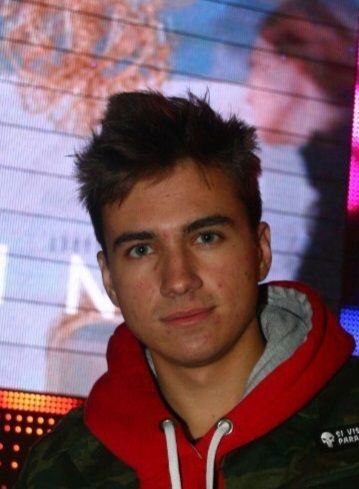
\includegraphics[scale=0.4]{img/avatar.jpg}
            };
        \end{tikzpicture}
    \end{center}
    \hfill
    \Huge % font size
    \sffamily 
    \begin{center} \color{\mainColor} \textbf{\MakeUppercase{#1}} \color{black} \textbf{#2} \end{center}\par % \par create a new paragraph
    \negxvspace
    \job{#3}
    \normalsize\normalfont % change the size and font back to normal
    \color{black} % change the color back to normal (black)
}

%%% Section Macro %%%

\newcommand{\cvsection}[2]{
    \section*{
        \color{\mainColor} \boxAwesome{#1} \negshspace \StrSplit{#2}{20}{\csA}{\csB} \csA\color{black}\csB
    }
}

%%% Subsection Macro %%%

\newcommand{\cvsubsection}[2]{
    \subsection*{
        \boxAwesome{#1} #2
    }
}

%%% Personal Details Macro %%%

\newcommand{\info}[2]{
  \noindent\hangindent=2em\hangafter=0 % \noindent delete default indentation ; \hangindent set custom indentation ; \hangafter indicate for how many lines we want this indentation (0 means for all lines)
  \boxAwesome{#1}
  #2 \par
  \svspace
}

\newcommand{\site}[1]{{\normalfont\sffamily\mdseries\small\color{grayShy}#1}}

%%% Skills Macro %%%

\newcommand{\simpleSkill}[1]{
    \noindent\hangindent=1.5em\hangafter=0
    \faAngleRight
    \shspace
    #1
    \svspace
    \par
}

\newcommand{\doubleSkill}[3]{
    \noindent\hangindent=1.5em\hangafter=0
    \parbox{30\spacebox} {
        \faAngleRight
        \boxAwesome{#1} \textbf{#2}
        \svspace
    } \svspace \texttt{#3} \par
}

%%% Work Experience Macro %%%

\newcommand{\work}[4]{
    \noindent \textbf{#1}
    \hfill % the following is written at the right of the document on the same line
    \framebox{
      \parbox{8em}{
      \centering\textbf{#2}
    }} \par
    \noindent \color{grayShy} \textsc{\MakeLowercase{#3}} \color{black} \par
    \noindent\hangindent=1.5em\hangafter=0 \textit{#4} \par
    \mvspace
    \normalsize \par
}

\newcommand{\workSubrole}[3]{
    \noindent \textbf{#1}
    \hfill
    \framebox{
      \parbox{8em}{
      \centering\textbf{#2}
    }} \par
    \noindent\hangindent=1.5em\hangafter=0 \textit{#3} \par
    \svspace
}

%%% Education Macro %%%

\newcommand{\education}[3]{
   \noindent \textbf{#1}
   \hfill
   \framebox{
      \parbox{8em}{
      \centering\textbf{#2}
    }} \par
    \noindent \color{grayShy} \textsc{\MakeLowercase{#3}} \color{black} \par
    \mvspace
    \normalsize \par
}

%%% Hobbies Macro %%%

\newcommand{\hobby}[2]{
    \noindent\hangindent=1.5em\hangafter=0
    \faAngleRight
    \shspace
    \boxAwesome{#1} #2
    \svspace
    \par
}

\newcommand{\projectTitle}[1]{
    \noindent\hangindent=1.5em\hangafter=0
    \faAngleRight
    \shspace
    {\normalsize\textbf{#1}} \par
    \negxvspace
}

\newcommand{\projectDesc}[1]{
    {\small #1 \par}
    \negxvspace
}

\newcommand{\projectTools}[1]{
    {\small \textit{\textbf{Tools:}} #1 \par}
    \mvspace
}

%%%%%%%%%%%%% Your CV below %%%%%%%%%%%%%

\begin{document}
    \name{Nikolay Tulupov}{}{4 year student, 21 y.o.}

    \info{\faEnvelopeOpen}{\texttt {tulupov.nd@phystech.edu}}
    \info{\faGithub}{\href{https://github.com/oncominglane}{\texttt{oncominglane}}}
    \info{\faVk}{\href{https://vk.com/oncoming_lane}{\texttt{vk.com/oncoming\_lane}}}
    \info{\faLink}{\href{https://t.me/oncoming_lane}{\texttt{t.me/oncoming\_lane}}}
        
    \negsvspace
    \cvsection{\faDna}{Skills}
    \svspace
    \cvsubsection{\faLaptopCode}{Technical skills}
    \svspace
    
    \doubleSkill{\faCode}{Programming languages}{C/C++ \textbullet{} Python \textbullet{} x86-64 assembly}
    
    \doubleSkill{\faTools}{Tools}{MATLAB \textbullet{} Motor-CAD \textbullet{} Git \textbullet{} CMake \textbullet{} ISE Design Suite \textbullet{} LaTeX}
    
    \doubleSkill{\faDesktop}{Devices}{Arduino \textbullet{} STM32 \textbullet{} RaspberryPi}

    \doubleSkill{\faMicrochip}{Embedded \& Interfaces}{UART \textbullet{} SPI \textbullet{} I2C \textbullet{} CAN \textbullet{} GPIO \textbullet{} ALSA}
    
    \doubleSkill{\faLinux}{OS}{Linux (Ubuntu, Armbian) \textbullet{} Windows}
    
    \doubleSkill{\faHammer}{Craft} {Soldering \textbullet{} Milling cutting \textbullet{} 3D printing \textbullet{} Laser cutting}
   
   

    \negsvspace
    \cvsubsection{\faHandsHelping}{Soft skills}
    \svspace

    \simpleSkill{Problem-solving in complex systems}
    \simpleSkill{Self-learning and fast adaptation}
    \simpleSkill{Technical communication}
    \simpleSkill{System thinking}
    

    \cvsection{\faGraduationCap}{Education}
    \svspace
    
    \education{Moscow Institute of Physics and Technology}{2022 - 2026}{Department of Radio Engineering and Computer Technologies}

    \cvsection{\faDesktop}{Work}
\svspace

\work{JSC PromSvyazRadio \href{http://prsvradio.ru/}{\site{prsvradio.ru}}}{02.2024 -- Present}{Assistant Engineer}{Support for radio equipment diagnostics, technical documentation, and coordination of engineering tasks.}

\noindent \textbf{JSC AMPEREMAGNETE \href{https://ampere.amtc.ru/ru/}{\site{ampere.amtc.ru/ru}}} \par
\noindent \color{grayShy} \textsc{\MakeLowercase{Engineering Intern}} \color{black} \par
\workSubrole{EV Controller Development Group}{09.2024 -- 03.2025}{Development of firmware logic for an AC charging-station controller board in accordance with the GB/T 18487 standard.}
\workSubrole{AI Development Group}{03.2025 -- 02.2026}{Optimization of electric drive control systems and firmware development for power inverters.}
\mvspace

\work{Moscow Institute of Physics and Technology \href{https://mipt.ru/education/basic-departments/kafedra-elektromobilnosti-i-magnitnykh-sistem}{\site{mipt.ru/.../kafedra-elektromobilnosti-i-magnitnykh-sistem}} \\ Robotics and Electric Drive Laboratory}{02.2026 -- Present}{Research Technician}{Optimization of electric drive control systems and preparation of scientific papers.}
    
    \neghvspace
    \cvsection{\faBook}{Projects}
    \svspace

\projectTitle{IPMSM Drive Control Optimization and Reinforcement Learning Research}
\projectDesc{Developed and validated methods for IPMSM drive control optimization: a new inverter torque-estimation approach, AT32-based inverter firmware, and real test-bench experiments. Also investigated reinforcement-learning-based control in simulation. A related paper is under review in \textit{eTransportation (Q1)}.}
\projectTools{C/C++, Python, Motor-CAD, embedded firmware, measurement bench}
    
\projectTitle{Remote Control System for Motorola XTL2500 Radio Station}
\projectDesc{Built a distributed client-server system on NaPi boards for remote radio control. Implemented real-time bidirectional audio, command handling, and SB9600/SBEP protocol interaction with frame parsing and display decoding. Integrated ADC/DAC and UART/SPI/I2C interfaces; currently finalizing PCB, enclosure, and documentation.}
\projectTools{C/C++, Linux, CMake, NaPi/Raspberry Pi, embedded interfaces, circuit design}
    
    
    \neghvspace
    \cvsection{\faPuzzlePiece}{Hobbies \& Interests}
    \svspace

    \hobby{\faTv}{Radio engineering}
    \hobby{\faGuitar}{Playing the guitar}
    \hobby{\faCar}{Cars and autosport}


\end{document}
